\documentclass[10pt, b5paper, openany]{ltjsbook}

\usepackage[T1]{fontenc}
\usepackage[utf8]{inputenc}
\usepackage[backend=biber, maxnames=100, backref=true]{biblatex}
\usepackage[binary-units = true]{siunitx}
\usepackage{amsmath, amssymb, amsthm}
\usepackage{graphicx}
\usepackage{hyperref}
\usepackage{ascmac}
\usepackage{here}
\usepackage{comment}
\usepackage{listings}

\setlength{\textwidth}{\fullwidth}
\setlength{\evensidemargin}{\oddsidemargin}

\lstset{
  basicstyle={\ttfamily},
  identifierstyle={\small},
  commentstyle={\smallitshape},
  keywordstyle={\small\bfseries},
  ndkeywordstyle={\small},
  stringstyle={\small\ttfamily},
  frame={tb},
  breaklines=true,
  columns=[l]{fullflexible},
  numbers=left,
  xrightmargin=0\zw,
  xleftmargin=3\zw,
  numberstyle={\scriptsize},
  stepnumber=1,
  numbersep=1\zw,
  lineskip=-0.5ex
}

\DeclareGraphicsRule{.ai}{pdf}{.ai}{}

\title{ \LaTeX Sample1 } 
\author{ komekome09(こめわっぽ) }
\date{ \today }

\begin{document} %document環境
\chapter*{はじめに}
みなさんはゲームをやっていますか?
PCでやるゲームと言えば、アクションゲーム、リズムゲーム、RPGなどがありますが、この本で扱うのはいわゆるノベルゲームと呼ばれるタイプのゲームについてです。

例えばみなさんは以下のような経験をしたことはありませんか?
\begin{itemize}
    \item 自宅のWindows機でやっているゲームを出先でもやりたいがMacしか持ってなくてできない……!
    \item Windowsしか対応してないけど宗教上の理由でWindowsが使えない… Vineだと動かないし…
\end{itemize}
こんなときにOSなどのプラットフォームに依存しないような実行環境があったら良いと思いませんか?
筆者は(学会などで遠出した際に)感じることがありました。

プラットフォーム非依存の環境で動作させるとなるとQtやJavaなどのクロスプラットフォームを採用しているソフトやライブラリで開発をすれば可能です。
しかし今までに発売されたソフトの中にはWindowsでしか動かないようなソフトも当然ありますし、それらのソフトに対する答えにはなりえません。

そこでこの本ではOSに依存しない環境で(主にWindows専用ソフトを対象とした)ノベルゲームを実行するためのプラットフォームを作ろうと奮闘した本です。
内容的にはまだまだですが、筆者が本を作ってみたいなどの個人的な都合などもあり、筆を取ることにしました。
本の内容としてはUEFIの基本的な内容から実際にどのように実装したのかまでを(なるべく)詳しく書いてみました。
誤字や誤記、間違いなどもあるかもしれませんが、見つけた時は遠慮なく教えていただけると幸いです。

\tableofcontents
\clearpage

\chapter{UEFIとは}
UEFIはUnified Extensible Firmware Interfaceの略で、OSとプラットフォームファームウェア間を結ぶインターフェースのことを指します。
一言で言うとBIOSの後継のようなものですが、BIOSから機能が大幅に拡張、変更されています。
BIOSでは基本的にOSのロードを行うブートローダーとしての役割がほとんどでしたが、UEFIではそのロードの前段階であらかじめ用意された多くの機能を扱うことができます。
また様々なハードウェア上で動作するように設計されているため、移植が比較的容易であるという利点もあります。
\footnote{もちろんハード依存の処理がある場合はその限りではありません。}

元々はIntelが1998年に開始したIntel Boot Initiativeが元になっており、2000年にEFIの仕様書が始めて作成されました。
\footnote{ただしこれは法的に問題があったため、2002年のバージョンアップからが正式となっています}
現在の最新バージョンは2.8です。

この本では、提供されるランタイム機能を駆使してUEFIアプリ(ノベルゲーム)を作成します。
そのUEFIアプリを作るのは別に仕様書を片手に全部1から書くことができますが、普通は開発用のツールが提供されています。
UEFIアプリでは主にEDK2とgnu-efiの2つが有名なツールです。

両者の大きな違いは機能の差です。
gnu-efiはUEFIのランタイムを扱う最低限の機能が提供されており、EDK2はこれに加えてmruby、libcなどのより高水準の機能が使えます。
この本ではgnu-efiを用いて開発を行っています。

\chapter{環境構築}
環境構築を行う前に、筆者の開発環境を下記に示します。
\begin{table}[H]
    \centering
    \begin{tabular}{|c|c|}
        \hline
        PC & MacBook Air (13-inch, Early 2015) \\
        CPU & Intel Core i5-5250U @ 1.60GHz \\
        Memory & 8GB \\
        OS & macOS Mojave 10.14.5 \\
        \hline
    \end{tabular}
\end{table}
macOSを使用していますが、コンパイルにはdockerを使うので他のOSでも動くと思います。

使用したソフト、ライブラリは、
\begin{itemize}
    \item gcc 8.2.0
    \item curl 7.63.0 (x86\_64)
    \item Docker Desktop Community Ver. 2.0.0.3 (31259)
    \item QEMU emulator version 4.0.0
    \item gnu-efi 3.0.9
\end{itemize}
です。

Dockerはなるべくホストの環境を汚さずに開発を行うために使っています。
DockerFileなどを含めたソースコード類はGitHubに上げています\footnote{\url{https://github.com/komekome09/efi-story}}。
今回は非常に軽量なAlpine Linux上にgnu-efiをビルドしています。

実行ファイルはPE32+形式ですが、クロスコンパイラ等は使用せずにコンパイルを行います。
まず普通にコンパイルを行い、その後生成されたファイルをobjcopyを用いてUEFIアプリケーションとして認識されるように書き換えています。

このコンテナではコンパイル部分のみを実行し、実際のコード編集と実行はホスト上で行うようにしています。
そのためコンテナとホストで開発ディレクトリを共有しています。
こうすることでホスト側の環境を汚すことなくコンパイルが可能になります。

この方法の他にもclangから直接PE32+形式のファイルを生成することも可能です。
その場合はDockerも必要なくなります(詳しくは\url{https://dvdhrm.github.io/2019/01/31/goodbye-gnuefi/}参照)。

QEMUでUEFIを扱うには、OVMF(Open Virtual Machine Hardware)と呼ばれるファームウェアを用いることで扱えるようにします。
OVMFはEDK2の一部として現在は配布されているなので
\footnote{\url{https://github.com/tianocore/edk2/tree/master/OvmfPkg}}
そこからダウンロードしますが、ビルドが必要になります。
今回はSourceForgeにあるビルド済のバイナリを用いています。
\footnote{\url{https://sourceforge.net/projects/edk2/files/OVMF/}}

コード編集から実行までの流れは、
\begin{enumerate}
    \item コードを編集する
    \item dockerコンテナを実行してコンパイル $\rightarrow$ 共有ディレクトリにファイルが生成される
    \item ホスト上で実行(今回はqemu)
\end{enumerate}
となります。

3段階に分かれてコマンドを叩くのは面倒なので、Makefileを用いてmakeコマンドのみで実行までできるようにしています。

\chapter{必要となる実装}
UEFIアプリ上でノベルゲームの土台を作るという目標ですが、具体的にどのような機能を実装すればいいのかを以下に示しました。
\begin{itemize}
    \item ファイル処理(読み書き)
    \item 画像処理(表示)
    \item BGM
    \item テキスト(フォント等)
    \item キー入力
\end{itemize}
まずはこれを足掛りとして考えていきます。

\section{ファイル処理}
ファイル処理はEFIインターフェースで提供されています。
そのため、仕様書に従って実装するだけで機能を実現できます。

\section{画像処理}
画像処理は表示するだけならEFIインターフェースで可能です。
表示には各ピクセルのRGBデータを得る必要がありますが、画像ファイルが圧縮されている場合などは解凍処理などを実装する必要があります。
また、透過処理(アルファブレンドなど)も実装が必要となります。
ノベルゲームなどでは図\ref{fig:nobel_exp}に示すようにテキストを表示する枠の部分(ピンク色)が背景画像(橙色)に対して透過していることが多々あるため、機能としては必須と考えています。
\begin{figure}[H]
    \centering
    \includegraphics[scale=0.3]{pic/nobel_exp.ai}
    \caption{ノベルゲームの表示例}
    \label{fig:nobel_exp}
\end{figure}

\section{BGM}
BGMに関してはUEFIが提供しているインターフェースに音楽などの再生機能が無いため、ドライバ経由でアクセスするなどの手段を自力で実装する必要があります。
実装方法としてはPCスピーカーを使う方法がもっとも単純ですが、いわゆるビープ音しか鳴らせないためHDA(High Difinition Audio)インターフェースに対応することでより高音質なデータを扱うことができます。
この本ではBGMに関しては述べません。

\section{テキスト}
インターフェース自体にも文字の出力関数は用意されていますが、画像で塗り潰してしまうため見えなくなるというのと、図\ref{fig:defaultfont}のように見栄えが非常に悪くなるという問題があります。
\begin{figure}[H]
    \centering
    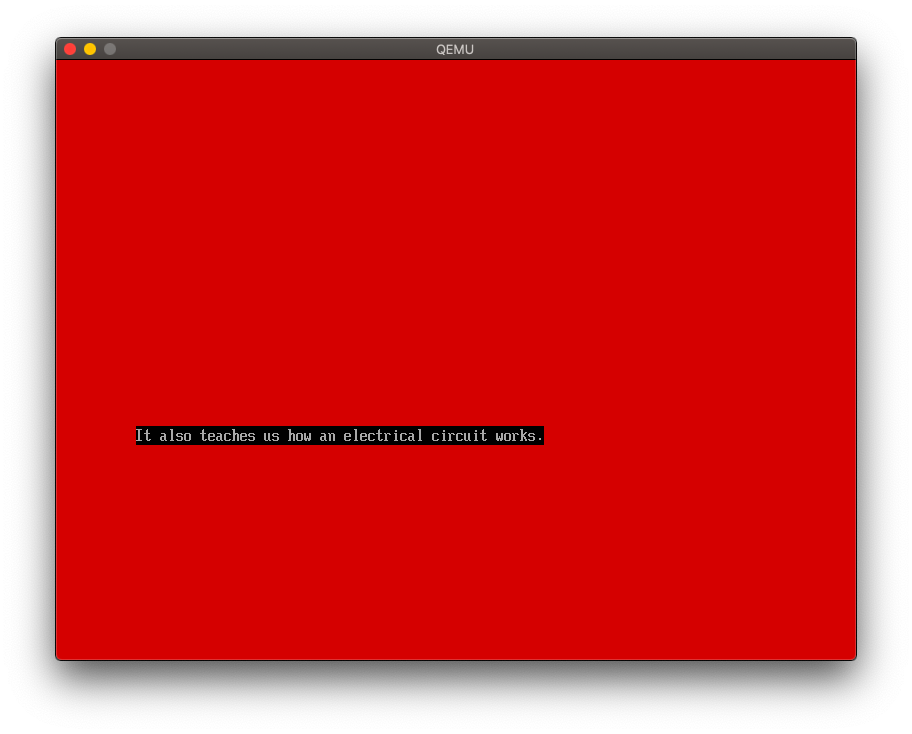
\includegraphics[scale=0.3]{pic/defaultfont.png}
    \caption{標準インターフェースでの文字の表示例}
    \label{fig:defaultfont}
\end{figure}
そのため、フォントを画像として表示することで各種問題を回避しています。
今回はGNU Unifontのビットマップ画像を用いたフォント表示を実装することにしました。
ビットマップフォントなので見た目はよろしくありませんが、背景色で透過できるためより自然な見た目になります。
将来的にはTrueTypeフォントを扱えるようにすることでより綺麗にフォントが表示することを考えています。

\chapter{コード}
\section{プログラミングをする上でのUEFI}
上で挙げた実装を実際のコードではどのように実現しているのかをこの項では書いていきますが、その前にUEFIランタイム(とgnu-efi)を扱う上で気をつけておく(自分が気になった)点を説明します。
\subsection{プロトコルとハンドラ}
一般的なプログラミング言語と同様に、UEFIのプロトコルもメモリ上にある関数へのポインタを経由して関数を呼び出しています。
その関数ポインタや識別するためのGUID、関数を使用するのに必要なデータ構造などをまとめた構造体がプロトコルと呼んでいるものです。
UEFI上ではこのプロトコルを使うためにはそのプロトコルのハンドラを取得し、そこからプロトコルを取得する必要があります。
gnu-efiではLibLocateProtocol関数を使うだけでプロトコルが使用可能な状態にしてくれますが、中身としてはハンドラの取得
\footnote{LocateHandle関数}
、プロトコルの取得
\footnote{HandleProtocol関数}
の2段階でプロトコルを取得しています。

\subsection{uefi\_call\_wrapper}
gnu-efiで関数を呼び出す際は
\begin{lstlisting}[caption=call function with gnu-efi,label=cfgnuefi]
uefi_call_wrapper(GraphicsOutput->Blt, 10, GraphicsOutput, BltBuffer, EfiBltBufferToVideo, 0, 0, 0, 0, DispWidth, DispHeight, DispWidth * sizeof(EFI_GRAPHICS_OUTPUT_BLT_PIXEL));
\end{lstlisting}
のように\verb+uefi_call_wrapper+関数を用いてラッパーとして呼び出します。
この\verb+uefi_call_wrapper+関数はABI(Application Binary Interface)の差異を吸収するためのマクロです。
コンパイルした後に生成されるファイルは機械語として出力されていますが、機械語に変換する際にABIは用いられます。
正確には使用しているデータ構造や処理内容が機械語ではどのように表わせるかを規定したものです。
\footnote{今回はMicrosoft ABIとSysv ABIの差異を吸収するのに用いられています。}
gnu-efiでは\verb+uefi_call_wrapper+マクロを使わないと呼び出せない場合があるので基本的にはこのマクロ経由で呼び出すようにしましょう。

\section{ファイル処理}
ファイルの処理には読み込む前にまずファイルが存在するディレクトリボリュームを開く必要があります。
ディレクトリボリュームは\verb+EFI_SIMPLE_FILE_SYSTEM_PROTOCOL+内のOpenVolume関数を用いて開きます。
必要となる部分だけ抜粋して載せます。
\begin{lstlisting}[caption=EFI\_SIMPLE\_FILE\_SYSTEM\_PROTOCOL,label=efi_simple_file_system_protocol]
typedef struct _EFI_SIMPLE_FILE_SYSTEM_PROTOCOL {
    UINT64 Revision;
    EFI_SIMPLE_FILE_SYSTEM_PROTOCOL_OPEN_VOLUME OpenVolume;
} EFI_SIMPLE_FILE_SYSTEM_PROTOCOL
\end{lstlisting}
\begin{lstlisting}[caption=EFI\_FILE\_PROTOCOL,label=efi_file_protocol]
typedef struct _EFI_FILE_PROTOCOL {
    UINT64         Revision;
    EFI_FILE_OPEN     Open;
    EFI_FILE_CLOSE     Close;
    EFI_FILE_DELETE    Delete;
    EFI_FILE_READ     Read;
    EFI_FILE_WRITE     Write;
    ︙
    } EFI_FILE_PROTOCOL;
\end{lstlisting}    
その後\verb+EFI_FILE_PROTOCOL+内のOpen関数でファイルを開き、先に確保したメモリ空間にRead関数を用いてデータを読み込みます。
ファイルサイズがOpenした状態では分からないため、ある程度の大きさのメモリ領域を確保した上で読み込み、その後メモリサイズをリサイズするという処理をしています。
\footnote{書いている途中にGetInfo関数で取れることに気づきました…}

\section{画像処理}
UEFI上での描画には、\verb+EFI_GRAPHICS_OUTPUT_PROTOCOL+というプロトコルを利用します。
\verb+EFI_GRAPHICS_OUTPUT_PROTOCOL+と\verb+EFI_GRAPHICS_OUTPUT_BLT_PIXEL+の構造を使用する部分だけ抜粋したのを以下に示します。
\begin{lstlisting}[caption=EFI\_GRAPHICS\_OUTPUT\_PROTOCOL,label=efi_gop]
typedef struct EFI_GRAPHICS_OUTPUT_PROTCOL {
    ︙
    EFI_GRAPHICS_OUTPUT_PROTOCOL_BLT        Blt;
    EFI_GRAPHICS_OUTPUT_PROTOCOL_MODE       *Mode;
} EFI_GRAPHICS_OUTPUT_PROTOCOL;
\end{lstlisting}
\begin{lstlisting}[caption=EFI\_GRAPHICS\_OUTPUT\_BLT\_PIXEL+,label=efi_gobp]
typedef struct {
    UINT8 Blue;
    UINT8 Green;
    UINT8 Red;
    UINT8 Reserved;
} EFI_GRAPHICS_OUTPUT_BLT_PIXEL;
\end{lstlisting}
このプロトコルには他にも2つの関数(QueryMode関数、SetMode関数)と1つの変数(Mode)があり、その中でも描画はBlt関数で行います。
具体的な描画プロセスは、1ピクセル毎のデータを表現する\verb+EFI_GRAPHICS_OUTPUT_BLT_PIXEL+構造体に代入し、それをフレームバッファーに描きこむことで描画します。
このフレームバッファーに描画する関数がBlt関数です。
\footnote{フレームバッファーに描画するだけでなく、読み込むことも出来ます。}
フレームバッファーにはアドレスを取得して直接書き込む方法もありますが、今回はダブルバッファリング(描画メモリと別のメモリ上との)を行うためBlt関数を使用しています。

画像ファイルは最初にRGBの生データに変換してから\verb+EFI_GRAPHICS_OUTPUT_BLT_PIXEL+構造体に代入します。
生データへの変換はnothings氏が作成したstbと呼ばれる単一ファイルから構成されるライブラリを利用しました。
\footnote{\url{https://github.com/nothings/stb} ライセンスはパブリックドメインです。}
このライブラリはlibcを利用しているため、libc関連の処理は全て置き換える必要があります。
変換した関数と置き換え後の関数の一覧を以下に示します。
\begin{table}[H]
    \centering
    \begin{tabular}{|c|c|}
        \hline
        置き換え前 & 置き換え後 \\
        \hline
        malloc & AllocatePool \\
        realloc & ReallocatePool \\
        free & FreePool \\
        memcpy & CopyMem \\
        memset & ZeroMem or SetMem \\
        \hline
    \end{tabular}
    \label{tb:function}
\end{table}
ここで挙げた置き換え後の関数は全部を網羅していませんが、最低限これだけの置き換えを行うことで動作しています。
また、全てUEFIのランタイム関数ではなくgnu-efi内で定義されている関数です。

処理の流れとしては以下のようになります。
\begin{itemize}
    \item ファイルの読み込み
    \item ライブラリを利用して別のメモリ領域に画像のRGBデータを読み込む
    \item フレームバッファに書き込み
    \item ディスプレイに描画
\end{itemize}
この処理を繰り返すことで描画を行います。

\section{フォント処理}
今回フォントの表示にはビットマップフォントを用いるので画像処理が出来ればフォント処理も同様に可能です。
ただしそのまま表示すると下の図のようにフォントの部分だけ背景が黒色になってしまうので、透過処理が必要になります。
\begin{figure}[H]
    \centering
    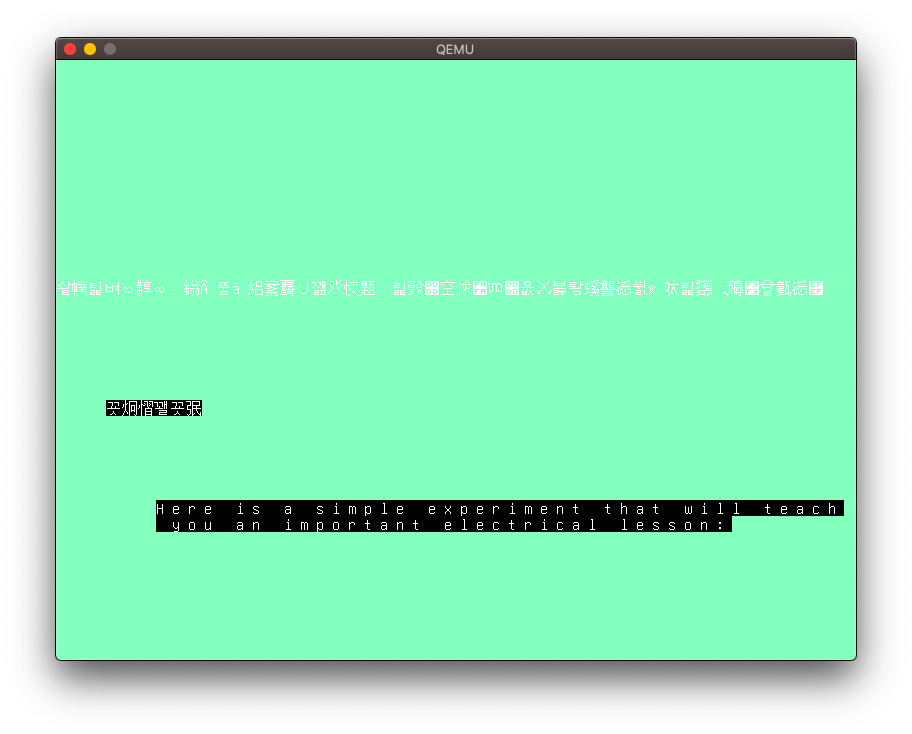
\includegraphics[scale=0.25]{pic/font_with_backblack.png}
    \caption{フォントの背景色を透過しなかった場合の結果}
    \label{fig:font_with_backblack}
\end{figure}
透過処理はRGBが指定した値以下であれば書き換えずに次のピクセルに移動するという非常に単純な処理です。

与えられた文字から画像データに変換するのにはUnicodeの符号位置をビットマップ上の位置に変換することで表示します。
UEFIでは標準で2バイトUnicodeを採用しているため、そこから上位ビットと下位ビットを抜き出すことで横軸上位ビット、縦軸下位ビットの組み合わせに落とし込むことが可能です。

\section{キー処理}
キー入力はReadKeyStroke関数を用いることで取得することが可能です。
ReadKeyStroke関数を実行すると\verb+EFI_INPUT_KEY+構造体に関数実行時点での入力キーが代入されます。
\verb+EFI_INPUT_KEY+構造体は以下のように定義されます。
\begin{lstlisting}[caption=EFI\_INPUT\_KEY,label=efi_input_key]
typedef struct {
    unsigned short ScanCode;
    unsigned short UnicodeChar;
} EFI_INPUT_KEY;
\end{lstlisting}
ScanCodeはUnicodeで表現できない文字が入力された場合に格納される変数です。
例えばEscキーが入力されるとScanCodeには0x17(23)が代入されます。
UTF-16で表現できる場合は0が代入されます。

UnicodeCharはScanCodeとは逆にUnicodeで表現できる文字が入力された場合に対応する文字を代入します。
Unicodeで表現できない文字の場合は0を代入します。

\chapter{あとがき}


\end{document}

